\documentclass[a4paper]{article}
\usepackage{geometry}
\usepackage{graphicx}
\usepackage{natbib}
\usepackage{amsmath}
\usepackage{amssymb}
\usepackage{amsthm}
\usepackage{paralist}
\usepackage{epstopdf}
\usepackage{tabularx}
\usepackage{longtable}
\usepackage{multirow}
\usepackage{multicol}
\usepackage[hidelinks]{hyperref}
\usepackage{fancyvrb}
\usepackage{algorithm}
\usepackage{algorithmic}
\usepackage{float}
\usepackage{paralist}
\usepackage[svgname]{xcolor}
\usepackage{enumerate}
\usepackage{array}
\usepackage{times}
\usepackage{url}
\usepackage{fancyhdr}
\usepackage{comment}
\usepackage{environ}
\usepackage{times}
\usepackage{textcomp}
\usepackage{caption}
%\usepackage{bbm}
\usepackage{dsfont}


\urlstyle{rm}

\setlength\parindent{0pt} % Removes all indentation from paragraphs
\theoremstyle{definition}
\newtheorem{definition}{Definition}[]
\newtheorem{conjecture}{Conjecture}[]
\newtheorem{example}{Example}[]
\newtheorem{theorem}{Theorem}[]
\newtheorem{lemma}{Lemma}
\newtheorem{proposition}{Proposition}
\newtheorem{corollary}{Corollary}

\floatname{algorithm}{Procedure}
\renewcommand{\algorithmicrequire}{\textbf{Input:}}
\renewcommand{\algorithmicensure}{\textbf{Output:}}
\newcommand{\abs}[1]{\lvert#1\rvert}
\newcommand{\norm}[1]{\lVert#1\rVert}
\newcommand{\RR}{\mathbb{R}}
\newcommand{\CC}{\mathbb{C}}
\newcommand{\Nat}{\mathbb{N}}
\newcommand{\br}[1]{\{#1\}}
\DeclareMathOperator*{\argmin}{arg\,min}
\DeclareMathOperator*{\argmax}{arg\,max}
\renewcommand{\qedsymbol}{$\blacksquare$}

\definecolor{dkgreen}{rgb}{0,0.6,0}
\definecolor{gray}{rgb}{0.5,0.5,0.5}
\definecolor{mauve}{rgb}{0.58,0,0.82}

\newcommand{\Var}{\mathrm{Var}}
\newcommand{\Cov}{\mathrm{Cov}}

\newcommand{\vc}[1]{\boldsymbol{#1}}
\newcommand{\xv}{\vc{x}}
\newcommand{\Sigmav}{\vc{\Sigma}}
\newcommand{\alphav}{\vc{\alpha}}
\newcommand{\muv}{\vc{\mu}}

\newcommand{\red}[1]{\textcolor{red}{#1}}

\def\x{\mathbf x}
\def\y{\mathbf y}
\def\w{\mathbf w}
\def\v{\mathbf v}
\def\E{\mathbb E}
\def\V{\mathbb V}
%\def\ind{\mathbbm 1}
\def\ind{\mathds 1}

% TO SHOW SOLUTIONS, include following (else comment out):
\newenvironment{soln}{
    \leavevmode\color{blue}\ignorespaces
}{}


\hypersetup{
%    colorlinks,
    linkcolor={red!50!black},
    citecolor={blue!50!black},
    urlcolor={blue!80!black}
}

\geometry{
  top=1in,            % <-- you want to adjust this
  inner=1in,
  outer=1in,
  bottom=1in,
  headheight=3em,       % <-- and this
  headsep=2em,          % <-- and this
  footskip=3em,
}


\pagestyle{fancyplain}
\lhead{\fancyplain{}{Homework 4}}
\rhead{\fancyplain{}{CS 760 Machine Learning}}
\cfoot{\thepage}

\title{\textsc{Homework 4}} % Title

%%% NOTE:  Replace 'NAME HERE' etc., and delete any "\red{}" wrappers (so it won't show up as red)

\author{
$>>$Sean(Xiaoyu) Sun$<<$\\
$>>$9078202463$<<$\\
} 

\date{}

\begin{document}

\maketitle 


\textbf{Instructions:} 
Although this is a programming homework, you only need to hand in a pdf answer file.
There is no need to submit the latex source or any code.
You can choose any programming language, as long as you implement the algorithm from scratch. 

Use this latex file as a template to develop your homework.
Submit your homework on time as a single pdf file to Canvas.
Please check Piazza for updates about the homework.

\section{Best Prediction Under 0-1 Loss (14 pts)}
Suppose the world generates a single observation $x \sim \mbox{multinomial}(\theta)$, where the parameter vector $\theta=(\theta_1, \ldots, \theta_k)$ with $\theta_i\ge 0$ and $\sum_{i=1}^k \theta_i=1$.  Note $x \in \{1, \ldots, k\}$.
You know $\theta$ and want to predict $x$. 
Call your prediction $\hat x$.  What is your expected 0-1 loss: 
$$\E \ind[\hat x \neq x]$$
using the following two prediction strategies respectively?  Prove your answer.

Strategy 1: $\hat x \in \argmax_x \theta_x$, the outcome with the highest probability.

\begin{soln}
Define $\max\theta$ is the maximum of $ \theta_k$ where $k \in \{1,2,...k\}$\\
$\E \ind[\hat x \neq x] = P(\hat x \neq x)\times1 = P(\max\theta \neq \theta_x) = 1 - P(\max\theta = \theta_x) = 1 - \max\theta$
\end{soln}

Strategy 2: You mimic the world by generating a prediction $\hat x \sim \mbox{multinomial}(\theta)$.  (Hint: your randomness and the world's randomness are independent)

\begin{soln}
$\E \ind[\hat x \neq x] = P(\hat x \neq x)\times1 = P(\theta_{\hat x} \neq \theta_x) = \sum_{i=1}^k{P(x = i, \hat x \neq i)} = \sum_{i=1}^k{\theta_i \times (1 - \theta_i)}$
\end{soln}

\section{Best Prediction Under Different Misclassification Losses (12 pts)}
Like in the previous question, 
the world generates a single observation $x \sim \mbox{multinomial}(\theta)$.
Let $c_{ij} \ge 0$ denote the loss you incur, if $x=i$ but you predict $\hat x=j$, for $i,j \in \{1, \ldots, k\}$.
$c_{ii}=0$ for all $i$.
This is a way to generalize different costs on false positives vs false negatives from binary classification to multi-class classification.
You want to minimize your expected loss:
$$\E c_{x \hat x}.$$
Derive your optimal prediction $\hat x$.

\begin{soln}
$ \hat x = \argmin_j \sum_{j=1}^k\sum_{i=1}^k{ c_{ij}\times P(x = i,\hat x = j) }$
\end{soln}

\section{Language Identification with Naive Bayes (8 pts each)}
Implement a character-based Naive Bayes classifier that classifies a document as English, Spanish, or Japanese - all written with the 26 lower case characters and space.

The dataset is languageID.tgz, unpack it.
This dataset consists of 60 documents in English, Spanish and Japanese. 
The correct class label is the first character of the filename: $y \in \{e, j, s\}$.

We will be using a character-based multinomial Naïve Bayes model.  You need to view each document as a bag of characters, including space.  We have made sure that there are only 27 different types of printable characters (a to z, and space) -- there may be additional control characters such as new-line, please ignore those.  Your vocabulary will be these 27 character types. (Note: not word types!)


\begin{enumerate}
\item
Use files 0.txt to 9.txt in each language as the training data.
Estimate the prior probabilities 
$\hat p(y=e)$,
$\hat p(y=j)$,
$\hat p(y=s)$
using add-1 smoothing. 
Give the formula for add-1 smoothing in this case. 
Print the prior probabilities.
(Hint: Store all probabilities here and below in $\log()$ internally to avoid underflow. This also means you need to do arithmetic in log-space.  But answer questions with probability, not log probability.)

\begin{soln}
all prior probabilities are $\frac{1}{3}$ (i.e. 0.3333333333333333 )
\end{soln}

\item
Using the same training data, estimate the class conditional probability (multinomial parameter) for English
$$\theta_{c,e} := \hat p(c \mid y=e)$$ 
for $c \in \{a, \ldots, z, space\}$.
Again use add-1 smoothing.
Give the formula for add-1 smoothing in this case. 
Print $\theta_e$ which is a vector with 27 elements.

\begin{soln}
$\theta_e =  $\\
$[0.060147893833355344, 0.01115806153439852, 0.021523834675821998, \\0.02198600290505744, 0.10530833223293279, 0.01894889739865311, \\0.017496368678198863, 0.047207183414762974, 0.05539416347550508, \\0.0014525287204542453, 0.003763369866631454, 0.028984550376336987, \\0.020533474184603197, 0.057903076719926054, 0.06443945596197016,\\ 0.01677010431797174, 0.0005942162947312822, 0.053809586689554996, \\0.06615608081341608, 0.08008715172322725, 0.026673709230159777, \\0.009309388617456754, 0.015515647695761256, 0.0011884325894625644, \\0.01386504687706325, 0.0006602403274792025, 0.17912320084510763]$

\end{soln}

\item
Print $\theta_j, \theta_s$.

\begin{soln}
$\theta_s =$\\
$[0.10450428245732947, 0.008256824203586173, 0.03752541746256701, \\0.0397436687411424, 0.11374699611806026, 0.008626532750015405, \\0.007209316655370016, 0.004559738739293857, 0.04984903567687473, \\0.006654753835726169, 0.000308090455357693, 0.05292994023045166, \\0.025817980158974674, 0.05416230205188243, 0.0724628751001294, \\0.02427752788218621, 0.007702261383942325, 0.059276603610820135, \\0.0657465031733317, 0.035615256639349314, 0.03370509581613162, \\0.005915336742867706, 0.00012323618214307722, 0.002526341733933083, \\0.007887115657156942, 0.0027111960071476986, 0.16815577053422884]$

$\theta_j = $\\
$[0.1316763247922921, 0.010891572994484396, 0.005515604272847867, \\0.017244990574600293, 0.06018292257208685, 0.0039097954339174755, \\0.01403337289673951, 0.031767087900579485, 0.09697689031627452, \\0.002373804370592753, 0.05739021154786009, 0.0014661732877190533, \\0.039796132095231446, 0.056692033791803396, 0.09111219716539831, \\0.0009076310828736997, 0.00013963555121133841, 0.042798296446275225, \\0.0421699364658242, 0.05697130489422607, 0.07058577113733157, \\0.00027927110242267683, 0.019758430496404383, 6.981777560566921e-05, \\0.014173008447950849, 0.007749773092229281, 0.12336800949521748]$
\end{soln}

\item
Treat e10.txt as a test document $x$.
Represent $x$ as a bag-of-words count vector (Hint: the vocabulary has size 27).
Print the bag-of-words vector $x$.

\begin{soln}
$[164, 32, 53, 57, 311, 55, 51, 140, 140, 3, 6, 85, 64, 139, 182, 53, 3, 141, 186, 225, 65, 31, 47, 4, 38, 2, 498]$
\end{soln}

\item
Compute $\hat p(x \mid y)$ for $y=e, j, s$ under the multinomial model assumption, respectively.
Use the formula
$$\hat p(x \mid y) = \prod_{i=1}^d \theta_{i, y}^{x_i}$$
where $x=(x_1, \ldots, x_d)$.
Show the three values: $\hat p(x \mid y=e), \hat p(x \mid y=j), \hat p(x \mid y=s)$.
Hint: you may notice that we omitted the multinomial coefficient.  This is ok for classification because it is a constant w.r.t. $y$.

\begin{soln}
$\hat p(x \mid y=e) =  e^ {-7841.786386770362}$\\
$\hat p(x \mid y=j) =  e^{-8452.383194656028}$\\
$\hat p(x \mid y=s) = e^{-8759.518886307718}$\\
\end{soln}

\item
Use Bayes rule and your estimated prior and likelihood, compute the posterior $\hat p(y \mid x)$.
Show the three values: $\hat p(y=e \mid x), \hat p(y=j \mid x), \hat p(y=s \mid x)$.
Show the predicted class label of $x$.

\begin{soln}
$P(x) = \hat p(x \mid y=e) \times \hat p(y=e)+\hat p(x \mid y=s) \times \hat p(y=s)+\hat p(x \mid y=j) \times \hat p(y=j) \\=   \frac{1}{3} \times (e^ {-7841.786386770362} +  e^{-8452.383194656028} +  e^{-8759.518886307718})$\\\\
$\hat p(y=e \mid x) = \frac{e^ {-7841.786386770362}}{3 \times P(x) }$\\
$\hat p(y=j \mid x) = \frac{e^{-8452.383194656028}}{3 \times P(x)}$\\
$\hat p(y=s \mid x) = \frac{e^{-8759.518886307718}}{3 \times P(x)}$\\

$\hat p(y=e \mid x) > \hat p(y=j \mid x) > \hat p(y=s \mid x)$\\
So the predicted class label of x should be 'e', which means x is an English file.
\end{soln}

\item
Evaluate the performance of your classifier on the test set (files 10.txt to 19.txt in three languages).
Present the performance using a confusion matrix. A confusion matrix summarizes the types of errors your classifier makes, as shown in the table below.   The columns are the true language a document is in, and the rows are the classified outcome of that document.  The cells are the number of test documents in that situation.  For example, the cell with row = English and column = Spanish contains the number of test documents that are really Spanish, but misclassified as English by your classifier.

\begin{center}
\begin{tabular}{c|ccc}
& English & Spanish & Japanese \\
\hline
English& 10 &0 &0 \\  
Spanish& 0& 10 &0\\ 
Japanese& 0& 0 & 10
\end{tabular}
\end{center}

\item Take a test document.   Arbitrarily shuffle the order of its characters so that the words (and spaces) are scrambled beyond human recognition.  How does this shuffling affect your Naive Bayes classifier's prediction on this document?  Explain the key mathematical step in the Naive Bayes model that justifies your answer.

\begin{soln}
Applying shuffle had no effect on the prediction. This is consistent with the mathmatical steps inside naive bayes algorithm.  Shuffle only changes every character's positional representation but naive bayes only takes the count of every character and has no positional representation of characters. So shuffle won't change anything of naive bayes's prediction.\\
\end{soln}

\end{enumerate}

\section{Weka (10 pts)}
Perform multinomial Naive Bayes classification.  Suggested key steps:
\begin{itemize}
\item We want you to experience Weka's TextDirectoryLoader.  For this, you need to prepare our documents such that each character becomes a word.  The easiest way is to insert a space between characters, but turn original space into the word ``space''.  For example, the document ``is the sun dying'' should be turned into ``i s space t h e space s u n space d y i n g''.
Then, create 3 subdirectories e, j, s and place each of the 20 documents in that language into the corresponding subdirectory.  
\item Find out how to ask Weka to use TextDirectoryLoader to load those 60 documents and use the subdirectory name as the class name.  This happens in the Preprocess tab in Weka Explorer.
\item Apply Filter: filters/unsupervised/Attribute/StringtoWordVec. Click to see options, set outputWordCounts to True (otherwise Weka uses binary absence/presence features, which is less interesting for our purpose). You should see @@class@@ and 27 features.
\item Choose Edit...  A big document by feature table will show up, where you should see word counts roughly in the range 1--100.  Right click on @@class@@, select ``Attribute as class''.  You may save it as an arff file.
The tri-color histogram for different features is interesting.
\item From the Classify tab, choose Classifier / bayes / NaiveBayesMultinomial
\item Let Weka perform 10-fold cross validation.  Report the resulting confusion matrix.

\begin{soln}
Weka gives perfect predictions of these files. (i.e. 100\% accuracy)\\
The results in detail are shown below:
	   \begin{figure}[H]
	        \centering
	        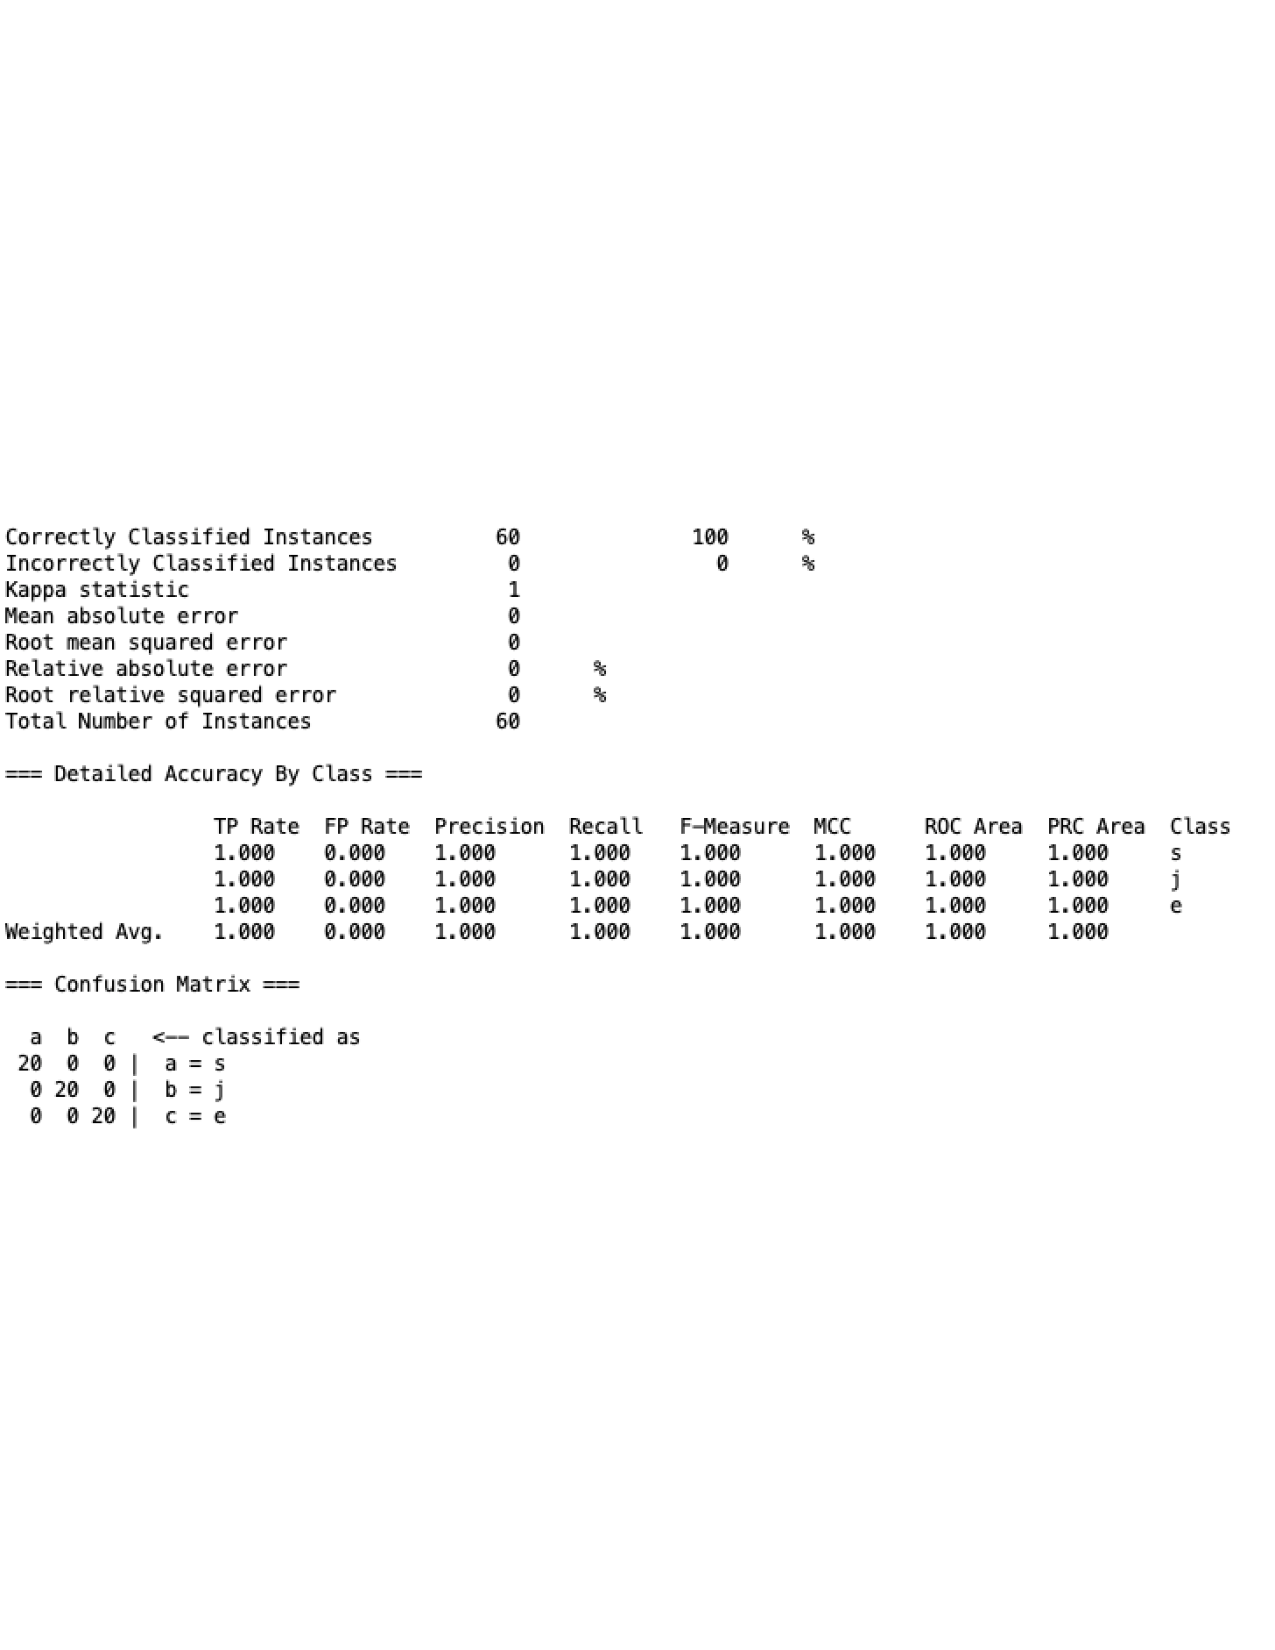
\includegraphics[width=1.0\textwidth]{result.pdf}
	        \captionsetup{labelformat=empty}
	        \caption{}
	        \label{fig:my_label}
	   \end{figure}
\end{soln}

\end{itemize}
\bibliographystyle{apalike}
\end{document}
